% Preamble
\documentclass[specialist,
  substylefile=spbu.rtx,
subf,href,colorlinks=true, 12pt]{disser}

% Packages
\usepackage[a4paper, includefoot,
  left=3cm, right=1.5cm,
  top=2cm, bottom=2cm,
headsep=1cm, footskip=1cm]{geometry}
\usepackage{amsmath}
\usepackage{amssymb}
\usepackage[T2A]{fontenc}
\usepackage[utf8]{inputenc}
\usepackage[english, russian]{babel}
\usepackage{pdfpages}
\usepackage{graphicx}
\usepackage{wrapfig}
\usepackage{amsthm}
\usepackage{framed}
\usepackage{xcolor}
\usepackage{color}
\usepackage{fancyvrb}
\usepackage{slashbox}
\usepackage{multirow}
\usepackage{mdwtab}
\usepackage{subcaption}
\usepackage{algorithm}
\usepackage{algorithmicx}
\usepackage{refcount}
\usepackage{placeins}
\usepackage{mathdots}

%new calligraphic font for subspaces 
\usepackage{euscript}
\newcommand{\cA}{\EuScript{A}}
\newcommand{\cB}{\EuScript{B}}
\newcommand{\cC}{\EuScript{C}}
\newcommand{\cD}{\EuScript{D}}
\newcommand{\cE}{\EuScript{E}}
\newcommand{\cF}{\EuScript{F}}
\newcommand{\cG}{\EuScript{G}}
\newcommand{\cH}{\EuScript{H}}
\newcommand{\cI}{\EuScript{I}}
\newcommand{\cJ}{\EuScript{J}}
\newcommand{\cK}{\EuScript{K}}
\newcommand{\cL}{\EuScript{L}}
\newcommand{\cM}{\EuScript{M}}
\newcommand{\cN}{\EuScript{N}}
\newcommand{\cO}{\EuScript{O}}
\newcommand{\cP}{\EuScript{P}}
\newcommand{\cQ}{\EuScript{Q}}
\newcommand{\cR}{\EuScript{R}}
\newcommand{\cS}{\EuScript{S}}
\newcommand{\cT}{\EuScript{T}}
\newcommand{\cU}{\EuScript{U}}
\newcommand{\cV}{\EuScript{V}}
\newcommand{\cW}{\EuScript{W}}
\newcommand{\cX}{\EuScript{X}}
\newcommand{\cY}{\EuScript{Y}}
\newcommand{\cZ}{\EuScript{Z}}

%font for text indices like transposition X^\mathrm{T}
\newcommand{\rmA}{\mathrm{A}}
\newcommand{\rmB}{\mathrm{B}}
\newcommand{\rmC}{\mathrm{C}}
\newcommand{\rmD}{\mathrm{D}}
\newcommand{\rmE}{\mathrm{E}}
\newcommand{\rmF}{\mathrm{F}}
\newcommand{\rmG}{\mathrm{G}}
\newcommand{\rmH}{\mathrm{H}}
\newcommand{\rmI}{\mathrm{I}}
\newcommand{\rmJ}{\mathrm{J}}
\newcommand{\rmK}{\mathrm{K}}
\newcommand{\rmL}{\mathrm{L}}
\newcommand{\rmM}{\mathrm{M}}
\newcommand{\rmN}{\mathrm{N}}
\newcommand{\rmO}{\mathrm{O}}
\newcommand{\rmP}{\mathrm{P}}
\newcommand{\rmQ}{\mathrm{Q}}
\newcommand{\rmR}{\mathrm{R}}
\newcommand{\rmS}{\mathrm{S}}
\newcommand{\rmT}{\mathrm{T}}
\newcommand{\rmU}{\mathrm{U}}
\newcommand{\rmV}{\mathrm{V}}
\newcommand{\rmW}{\mathrm{W}}
\newcommand{\rmX}{\mathrm{X}}
\newcommand{\rmY}{\mathrm{Y}}
\newcommand{\rmZ}{\mathrm{Z}}

%tt font for time series
\newcommand{\tA}{\mathsf{A}}
\newcommand{\tB}{\mathsf{B}}
\newcommand{\tC}{\mathsf{C}}
\newcommand{\tD}{\mathsf{D}}
\newcommand{\tE}{\mathsf{E}}
\newcommand{\tF}{\mathsf{F}}
\newcommand{\tG}{\mathsf{G}}
\newcommand{\tH}{\mathsf{H}}
\newcommand{\tI}{\mathsf{I}}
\newcommand{\tJ}{\mathsf{J}}
\newcommand{\tK}{\mathsf{K}}
\newcommand{\tL}{\mathsf{L}}
\newcommand{\tM}{\mathsf{M}}
\newcommand{\tN}{\mathsf{N}}
\newcommand{\tO}{\mathsf{O}}
\newcommand{\tP}{\mathsf{P}}
\newcommand{\tQ}{\mathsf{Q}}
\newcommand{\tR}{\mathsf{R}}
\newcommand{\tS}{\mathsf{S}}
\newcommand{\tT}{\mathsf{T}}
\newcommand{\tU}{\mathsf{U}}
\newcommand{\tV}{\mathsf{V}}
\newcommand{\tW}{\mathsf{W}}
\newcommand{\tX}{\mathsf{X}}
\newcommand{\tY}{\mathsf{Y}}
\newcommand{\tZ}{\mathsf{Z}}

%bf font for matrices
\newcommand{\bfA}{\mathbf{A}}
\newcommand{\bfB}{\mathbf{B}}
\newcommand{\bfC}{\mathbf{C}}
\newcommand{\bfD}{\mathbf{D}}
\newcommand{\bfE}{\mathbf{E}}
\newcommand{\bfF}{\mathbf{F}}
\newcommand{\bfG}{\mathbf{G}}
\newcommand{\bfH}{\mathbf{H}}
\newcommand{\bfI}{\mathbf{I}}
\newcommand{\bfJ}{\mathbf{J}}
\newcommand{\bfK}{\mathbf{K}}
\newcommand{\bfL}{\mathbf{L}}
\newcommand{\bfM}{\mathbf{M}}
\newcommand{\bfN}{\mathbf{N}}
\newcommand{\bfO}{\mathbf{O}}
\newcommand{\bfP}{\mathbf{P}}
\newcommand{\bfQ}{\mathbf{Q}}
\newcommand{\bfR}{\mathbf{R}}
\newcommand{\bfS}{\mathbf{S}}
\newcommand{\bfT}{\mathbf{T}}
\newcommand{\bfU}{\mathbf{U}}
\newcommand{\bfV}{\mathbf{V}}
\newcommand{\bfW}{\mathbf{W}}
\newcommand{\bfX}{\mathbf{X}}
\newcommand{\bfY}{\mathbf{Y}}
\newcommand{\bfZ}{\mathbf{Z}}

%bb font for standard spaces and expectation
\newcommand{\bbA}{\mathbb{A}}
\newcommand{\bbB}{\mathbb{B}}
\newcommand{\bbC}{\mathbb{C}}
\newcommand{\bbD}{\mathbb{D}}
\newcommand{\bbE}{\mathbb{E}}
\newcommand{\bbF}{\mathbb{F}}
\newcommand{\bbG}{\mathbb{G}}
\newcommand{\bbH}{\mathbb{H}}
\newcommand{\bbI}{\mathbb{I}}
\newcommand{\bbJ}{\mathbb{J}}
\newcommand{\bbK}{\mathbb{K}}
\newcommand{\bbL}{\mathbb{L}}
\newcommand{\bbM}{\mathbb{M}}
\newcommand{\bbN}{\mathbb{N}}
\newcommand{\bbO}{\mathbb{O}}
\newcommand{\bbP}{\mathbb{P}}
\newcommand{\bbQ}{\mathbb{Q}}
\newcommand{\bbR}{\mathbb{R}}
\newcommand{\bbS}{\mathbb{S}}
\newcommand{\bbT}{\mathbb{T}}
\newcommand{\bbU}{\mathbb{U}}
\newcommand{\bbV}{\mathbb{V}}
\newcommand{\bbW}{\mathbb{W}}
\newcommand{\bbX}{\mathbb{X}}
\newcommand{\bbY}{\mathbb{Y}}
\newcommand{\bbZ}{\mathbb{Z}}

%got font for any case
\newcommand{\gA}{\mathfrak{A}}
\newcommand{\gB}{\mathfrak{B}}
\newcommand{\gC}{\mathfrak{C}}
\newcommand{\gD}{\mathfrak{D}}
\newcommand{\gE}{\mathfrak{E}}
\newcommand{\gF}{\mathfrak{F}}
\newcommand{\gG}{\mathfrak{G}}
\newcommand{\gH}{\mathfrak{H}}
\newcommand{\gI}{\mathfrak{I}}
\newcommand{\gJ}{\mathfrak{J}}
\newcommand{\gK}{\mathfrak{K}}
\newcommand{\gL}{\mathfrak{L}}
\newcommand{\gM}{\mathfrak{M}}
\newcommand{\gN}{\mathfrak{N}}
\newcommand{\gO}{\mathfrak{O}}
\newcommand{\gP}{\mathfrak{P}}
\newcommand{\gQ}{\mathfrak{Q}}
\newcommand{\gR}{\mathfrak{R}}
\newcommand{\gS}{\mathfrak{S}}
\newcommand{\gT}{\mathfrak{T}}
\newcommand{\gU}{\mathfrak{U}}
\newcommand{\gV}{\mathfrak{V}}
\newcommand{\gW}{\mathfrak{W}}
\newcommand{\gX}{\mathfrak{X}}
\newcommand{\gY}{\mathfrak{Y}}
\newcommand{\gZ}{\mathfrak{Z}}

%old calligraphic font
\newcommand{\calA}{\mathcal{A}}
\newcommand{\calB}{\mathcal{B}}
\newcommand{\calC}{\mathcal{C}}
\newcommand{\calD}{\mathcal{D}}
\newcommand{\calE}{\mathcal{E}}
\newcommand{\calF}{\mathcal{F}}
\newcommand{\calG}{\mathcal{G}}
\newcommand{\calH}{\mathcal{H}}
\newcommand{\calI}{\mathcal{I}}
\newcommand{\calJ}{\mathcal{J}}
\newcommand{\calK}{\mathcal{K}}
\newcommand{\calL}{\mathcal{L}}
\newcommand{\calM}{\mathcal{M}}
\newcommand{\calN}{\mathcal{N}}
\newcommand{\calO}{\mathcal{O}}
\newcommand{\calP}{\mathcal{P}}
\newcommand{\calQ}{\mathcal{Q}}
\newcommand{\calR}{\mathcal{R}}
\newcommand{\calS}{\mathcal{S}}
\newcommand{\calT}{\mathcal{T}}
\newcommand{\calU}{\mathcal{U}}
\newcommand{\calV}{\mathcal{V}}
\newcommand{\calW}{\mathcal{W}}
\newcommand{\calX}{\mathcal{X}}
\newcommand{\calY}{\mathcal{Y}}
\newcommand{\calZ}{\mathcal{Z}}


\setcounter{tocdepth}{2}
\graphicspath{{../img}}

\theoremstyle{plain}
\newtheorem{statement}{Утверждение}[section]
\newtheorem{theorem}{Теорема}

\theoremstyle{definition}
\newtheorem{definition}{Определение}[section]
\newtheorem{property}{Свойство}[section]
\newtheorem{example}{Пример}[section]
\newtheorem*{corollary}{Следствие}

\theoremstyle{remark}
\newtheorem*{remark}{Замечание}

\newcommand{\Input}{\textbf{Входные данные: }}
\newcommand{\Output}{\textbf{Результат: }}
\newcommand{\iu}{\mathrm{i}}

\floatname{algorithm}{Алгоритм}
\renewcommand{\listalgorithmname}{Список алгоритмов}

% Document
\begin{document}\section{Известные сведения об алгоритмах SSA и MSSA}\label{sec:known-results-ssa}
В этом разделе приведены описания алгоритмов SSA и MSSA, а также некоторые их свойства и важные определения.

\subsection{SSA}\label{subsec:ssa}
Все определения и утверждения из этого раздела можно найти в книге~\cite{ssa}.

Пусть дан временной ряд $\tX$ длины $N$
\[
  \tX=(x_1,x_2,\ldots,x_N).
\]

\begin{definition}[Оператор вложения]
  \label{def:injection-op}
  Оператором вложения $\calH_L$ с длиной окна $L$ будем называть отображение, переводящее временной ряд
  $\tX=(x_1, x_2,\ldots, x_N)$, $N \geqslant L$, в ганкелеву матрицу $\bfX\in \bbR^{L \times K}$, $K = N-L+1$,
  такую, что $\bfX_{lk}=x_{l+k-1}$.
  Результирующая матрица имеет вид
  \[
    \calH_L(\tX) = \bfX =
    \begin{pmatrix}
      x_1    & x_2     & \ldots & x_K     \\
      x_2    & x_3     & \ldots & x_{K+1} \\
      \vdots & \vdots  & \ddots & \vdots  \\
      x_L    & x_{L+1} & \ldots & x_N
    \end{pmatrix}.
  \]
\end{definition}

\begin{definition}[Траекторная матрица]
  Траекторной матрицей ряда $\tX$ с длиной окна $L<N$ называют матрицу $\bfX$, полученную применением оператора
  вложения $\calH_L$, к ряду $\tX$.
\end{definition}

Пусть временной ряд $\tX$ представим в виде суммы временных рядов $\tX_k$ и шума $\tE$:
\[
  \tX = \sum_{k=1}^{m} \tX_k + \tE.
\]
В алгоритме~\ref{alg:ssa-components} описан метод SSA для разделения компонент сигнила, то есть
нахождения рядов $\tX_k$.
В алгоритме~\ref{alg:ssa-signal} описан метод SSA для выделения сигнала, то есть нахождения $\sum_{k=1}^{m} \tX_k$.
Первые два шага в алгоритме~\ref{alg:ssa-signal} совпадают с соответствующими шагами
алгоритма~\ref{alg:ssa-components}, поэтому описание алгоритма начинается с шага 3.

\begin{algorithm}[!h]
  \caption{SSA для разделения компонент сигнала.}
  \label{alg:ssa-components}
  \Input $\tX$, $L: 1 < L < N$, где $N$ "--- длина $\tX$, $m$, $R: m \leqslant R\leqslant \min(L, N-L+1)$,
  $\mathfrak{S}_1, \ldots, \mathfrak{S}_m$:
  \[
    \{1,\, 2\,\ldots,\, R\}=\bigcup_{k=1}^{m}\mathfrak{S}_k, \qquad \mathfrak{S}_k\cap \mathfrak{S}_l =\varnothing,\,
    k\ne l.
  \]
  \Output $\widetilde{\tX}_1$, $\widetilde{\tX}_2$, $\ldots$, $\widetilde{\tX}_m$ "--- оценки рядов
  $\tX_1$, $\tX_2$, $\ldots$, $\tX_m$.
  \begin{algorithmic}[1]
    \State Вложение: построение траекторной матрицы $\bfX$ по длине окна $L$.
    \State Разложение: проведение SVD траекторной матрицы $\bfX$, получение её представления в виде
    \begin{equation*}
      \bfX=\sum_{i=1}^{d} \sqrt{\lambda_i} U_i V_i^{\rmT}, \quad R \leqslant d \leqslant \min(L, N-L+1).
    \end{equation*}
    \State Группировка: построение матриц
    \begin{equation*}
      \bfX_k=\sum_{i \in \mathfrak{S}_k} \sqrt{\lambda_i} U_i V_i^{\rmT}.
      %            \label{eq:tens-group}
    \end{equation*}
    \State Восстановление: вычисление рядов $\widetilde{\tX}_k$ по матрицам $\bfX_k$ посредством их усреднения
    вдоль побочных диагоналей $i + j =\operatorname{const}$:
    \begin{gather*}
      \tilde{x}^{(k)}_n=\frac{1}{\#\mathfrak{M}_n}\sum_{(i,j)\in \mathfrak{M}_n}
      \left(\bfX_k\right)_{ij},\qquad n\in \overline{1:N},\\
      \mathfrak{M}_n=\left\{(i,\, j)~\Big|~1\leqslant i \leqslant L,\, 1\leqslant j \leqslant N-L+1,\,
      i+j-1=n\right\}.
    \end{gather*}
  \end{algorithmic}
\end{algorithm}

\begin{algorithm}[!h]
  \caption{SSA для выделения сигнала.}
  \label{alg:ssa-signal}
  \Input $\tX$, $L: 1 < L < N$, где $N$ "--- длина $\tX$, $R: 1 \leqslant R\leqslant \min(L, N-L+1)$.\\
  \Output $\widetilde{\tX}$ "--- оценка сигнала $\sum_{k=1}^{m} \tX_k$.
  \begin{algorithmic}[1]
    \setcounter{ALG@line}{2}
    %            \State Построение траекторной матрицы $\bfX$ по длине окна $L$.
    %            \State Проведение SVD траекторной матрицы $\bfX$, получение её представления в виде
    %            \begin{equation*}
    %                \bfX=\sum_{i=1}^{d} \sqrt{\lambda_i} U_i V_i^{\rmT}, \quad R \leqslant d \leqslant \min(L, N-L+1).
    %            \end{equation*}
    \State Группировка: построение матрицы
    \begin{equation*}
      \widetilde{\bfX} = \sum_{i = 1}^{R} \sqrt{\lambda_i} U_i V_i^{\rmT}.
      %            \label{eq:tens-group}
    \end{equation*}
    \State Восстановление ряда $\widetilde{\tX}$ по матрице $\widetilde{\bfX}$ посредством её усреднения
    вдоль побочных диагоналей $i + j =\operatorname{const}$.
  \end{algorithmic}
\end{algorithm}

\begin{definition}[SSA-ранг временного ряда]
  \label{def:ssa-rank}
  Число $d$ называется SSA-рангом временного ряда $\tX$ длины $N$, если $d \leqslant (N+1) / 2$ и для любой допустимой
  длины окна $L$,
  то есть такой, что $d \leqslant \min(L, N- L + 1)$, ранг траекторной матрицы $\bfX$ этого ряда, построенной по
  длине окна $L$, равен $d$.
\end{definition}
\begin{remark}
  В качестве параметра $R$ в алгоритмах~\ref{alg:ssa-components} и~\ref{alg:ssa-signal} рекомендуется выбирать
  SSA-ранг сигнала.
\end{remark}

\begin{example}
  \label{ex:ssa-ranks}
  Ниже приведены примеры некоторых рядов, имеющих конечные SSA-ранги.
  \begin{itemize}
    \item Ранг полиномиального ряда $x_n = Q_d(n)$, где $Q_d$ "--- многочлен степени $d$, равен $d + 1$.
    \item Ранг экспоненциального ряда $x_n = C e^{\alpha n}$, где $\alpha \in \bbC$ и $C \ne 0$, равен 1.
    \item Ранг суммы экспоненциальных рядов
      \[
        x_n = \sum_{j=1}^{M} C_j e^{\alpha_j n},
      \]
      где $\alpha_j \in \bbC$ и $C_j \ne 0$ при всех $j$, равен количеству уникальных
      значений $\alpha_j$.
    \item Ранг экспоненциально-модулированного гармонического ряда
      \[
        x_n = C e^{\alpha n}\cos(2 \pi n \omega + \psi),
      \]
      где $C \ne 0$, $\alpha \in \bbR$ и $\omega \in [0,1/2]$,
      равен $r(\omega)$, где
      \begin{equation}
        \label{eq:cos-rank}
        r(\omega) =
        \begin{cases}
          1, & \omega \in \{0,\, 1/2\},\\
          2, & \omega \in (0, 1/2).
        \end{cases}
      \end{equation}
    \item Ранг суммы экспоненциально-модулированных гармоник
      \[
        x_n = \sum_{j=1}^{M} C e^{\alpha_j n}\cos(2 \pi n \omega_j + \psi_j)
      \]
      равен
      \begin{equation*}
        \label{eq:cos-sum-rank}
        \sum_{(\omega, \alpha)\in \Omega} r(\omega),
      \end{equation*}
      где $\Omega$ "--- множество уникальных пар $(\omega_i,\, \alpha_i)$, представленных в данном временном ряде.
  \end{itemize}
\end{example}

\begin{definition}[Слабая SSA-разделимость]
  \label{def:ssa-separability}
  Временные ряды $\widehat{\tX} = (\hat{x}_1, \hat{x}_2, \ldots, \hat{x}_N)$ и
  $\widetilde{\tX} = (\tilde{x}_1, \tilde{x}_2, \ldots, \tilde{x}_N)$ называют слабо $L$-разделимыми в терминах
  SSA, если выполнены следующие условия:
  \begin{enumerate}
    \item $\displaystyle \sum_{k=0}^{L - 1} \hat{x}_{i + k}\tilde{x}_{j + k} = 0,
      \quad \forall i, j \in \overline{1:(N - L + 1)}$,
    \item $\displaystyle \sum_{k=0}^{N - L} \hat{x}_{i + k}\tilde{x}_{j + k} = 0,
      \quad \forall i, j \in \overline{1:L}$.
  \end{enumerate}
\end{definition}

\begin{statement}
  \label{state:ssa-separability}
  Пусть $\tX = \widehat{\tX} + \widetilde{\tX}$, а $\bfX$, $\widehat{\bfX}$ и $\widetilde{\bfX}$ "--- траекторные
  матрицы с длиной окна $L$ рядов $\tX$, $\widehat{\tX}$ и $\widetilde{\tX}$ соответственно.
  Тогда сумма \emph{SVD} матриц $\widehat{\bfX}$ и $\widetilde{\bfX}$ является \emph{SVD} матрицы $\bfX$ тогда и только тогда, когда
  ряды $\widehat{\tX}$ и $\widetilde{\tX}$ слабо $L$-разделимы в терминах \emph{SSA}.
\end{statement}

Утверждение~\ref{state:ssa-separability} позволяет выделить множество временных рядов, которые возможно
разделить алгоритмом~\ref{alg:ssa-components}, а именно: слабо разделимые с некоторой длиной окна.

\subsection{MSSA}\label{subsec:mssa}
Все определения и утверждения из этого раздела можно найти в работах~\cite{mssa, mssa2, ssa-2020}.

Пусть дан $P$-мерный временной ряд $\tX$ длины $N$
\begin{gather*}
  \tX = (\tX_1: \tX_2: \ldots: \tX_P), \\
  \tX_p = \left(x_1^{(p)}, x_2^{(p)}, \ldots, x_N^{(p)}\right)^{\rmT}.
\end{gather*}

\begin{definition}[Траекторная матрица многомерного временного ряда]
  Пусть \linebreak $\bfX_1$, $\bfX_2$, $\ldots$, $\bfX_P$ "--- траекторные матрицы рядов
  $\tX_1$, $\tX_2$, $\ldots$, $\tX_P$ соответственно, построенные по длине окна $L$.
  Траекторной матрицей многомерного временного ряда $\tX$ называется
  матрица $\bfX\in \bbR^{L \times KP}$, $K = N - L + 1$, построенная соединением матриц $\bfX_p$ по столбцам, то есть
  \[
    \bfX = [\bfX_1 : \bfX_2 : \ldots : \bfX_P].
  \]
\end{definition}

Методы MSSA для разделения компонент и выделения сигнала совпадают с алгоритмами~\ref{alg:ssa-components}
и~\ref{alg:ssa-signal} соответственно, с точностью до изменения шагов вложения и восстановления в соответствии
с определением траекторной матрицы многомерного ряда (процедура восстановления временного ряда по
матрице должна быть обратной к шагу вложения).

\begin{definition}[MSSA-ранг временного ряда]
  \label{def:mssa-rank}
  Число $d$ называется MSSA-рангом $P$-мерного временного ряда $\tX$ длины $N$, если $d \leqslant P(N+1) / (P+1)$,
  и для любой допустимой
  длины окна $L$,
  то есть такой, что $d \leqslant \min(L, P(N- L + 1))$, ранг траекторной матрицы $\bfX$ этого ряда,
  построенной по длине окна $L$, равен $d$.
\end{definition}
\begin{remark}
  Как и в SSA, в алгоритме MSSA рекомендуется в качестве параметра количества компонент, относимых к сигналу,
  выбирать ранг сигнала.
\end{remark}
\begin{example}
  \label{ex:mssa-ranks}
  Рассмотрим $P$-мерный временной ряд $\tX$ длины $N$ с элементами вида
  \begin{equation}
    \label{eq:nd-cos-sum-model}
    x_n^{(p)} = \sum_{i=1}^{R(p)} a_i^{(p)} e^{-\alpha_i^{(p)} n}
    \cos\left(2 \pi \omega_i^{(p)} n + \varphi_i^{(p)}\right).
  \end{equation}
  MSSA-ранг такого ряда равен
  \begin{equation}
    \sum_{(\omega, \alpha)\in \Omega} r(\omega),
  \end{equation}
  где функция $r(\omega)$ определена в уравнении~\eqref{eq:cos-rank}, а $\Omega$ "--- множество уникальных пар
  \linebreak $\left(\omega_i^{(p)}, \alpha_i^{(p)}\right)$, представленных в данном временном ряде.
\end{example}

\begin{remark}
  В дальнейшем в работе будут проведены сравнения методов SSA и MSSA с их тензорными модификациями
  HO-SSA и HOSVD-MSSA на многомерных сигналах вида~\eqref{eq:nd-cos-sum-model}.
  Это обосновано тем, что такая модель, а точнее её частный случай, в котором параметры $R(p)$, $\omega_i^{(p)}$
  и $\alpha_i^{(p)}$ не зависят от номера ряда $p$, применяется в спектроскопии ядерного магнитного
  резонанса~\cite{NMR}.
  Кроме того, в работе~\cite{hosvd-hooi-separation} также рассматривается этот частный случай модели.
\end{remark}

\begin{definition}[Слабая MSSA-разделимость]
  \label{def:mssa-separability}
  $P$-мерные временные ряды $\widehat{\tX}$ и $\widetilde{\tX}$ длины $N$ называются слабо $L$-разделимыми, если
  выполнены следующие условия:
  \begin{enumerate}
    \item $\displaystyle \sum_{k=0}^{L-1} \hat{x}_{i+k}^{(p)}\tilde{x}_{j+k}^{(p')} = 0,
      \qquad \forall i, j \in \overline{1:(N-L+1)},\, p, p' \in \overline{1:P}$,
    \item $\displaystyle \sum_{p=1}^{P} \sum_{i=0}^{K-1} \hat{x}_{k+i}^{(p)} \tilde{x}_{m+i}^{(p)} = 0, \quad
      \forall k, m \in \overline{1:L}$.
  \end{enumerate}
\end{definition}

\begin{statement}
  \label{state:mssa-separability}
  Пусть $\tX = \widehat{\tX} + \widetilde{\tX}$, а $\bfX$, $\widehat{\bfX}$ и $\widetilde{\bfX}$ "--- траекторные
  матрицы с длиной окна $L$ рядов $\tX$, $\widehat{\tX}$ и $\widetilde{\tX}$ соответственно.
  Тогда сумма \emph{SVD} матриц $\widehat{\bfX}$ и $\widetilde{\bfX}$ является \emph{SVD} матрицы $\bfX$ тогда и только тогда, когда
  ряды $\widehat{\tX}$ и $\widetilde{\tX}$ слабо $L$-разделимы в терминах MSSA.
\end{statement}
Как и в одномерном случае, это утверждение позволяет определять множество рядов, которые возможно разделить с
помощью метода MSSA.

\subsection{ESPRIT}\label{subsec:esprit}
Оригинальное описание алгоритма и его обоснование
можно найти в статьях~\cite{esprit,hosvd-hooi-separation}.

Пусть элементы многомерного временного ряда $\tX$ имеют вид
\begin{equation}
  \label{eq:esprit-model}
  x_n^{(p)} = \sum_{j=1}^{R} a_j^{(p)} e^{ \alpha_j n }
  e^{\iu \left( 2 \pi \omega_j n + \varphi_j^{(p)}\right)},
\end{equation}
где $\iu$ обозначает мнимую единицу, а параметрами модели являются амплитуды
$a_j^{(p)} \in \mathbb{R}\setminus\{0\}$, фазы ${\varphi_j^{(p)} \in [0, 2\pi)}$,
частоты $\omega_j\in [0, 1/2]$ и степени затухания $\alpha_j \in \mathbb{R}$.

\begin{remark}
  В статье~\cite{esprit} приводится алгоритм ESPRIT для модели временного ряда вида
  \[
    x_n^{(p)} = \sum_{j=1}^{R} s_j(n)e^{\iu \omega_0 \Delta \sin\theta_j / c} a^{(p)}(\theta_j),
  \]
  где оцениваемые параметры обозначены $\theta_j$,
  но в работе будет рассматриваться модель вида~\eqref{eq:esprit-model} по причине,
  указанной в замечании к примеру~\ref{ex:mssa-ranks}.
\end{remark}
\begin{remark}
  В силу того, что
  \[
    \cos(2 \pi \omega n + \varphi_n) =
    \frac{e^{2\pi \iu \omega n + \varphi_n} + e^{-2\pi \iu \omega n - \varphi_n}}{2},
  \]
  вещественнозначный временной ряд из примера~\ref{ex:mssa-ranks} при
  $R(p)=R$, $\omega_j^{(p)}=\omega_j$ и $\alpha_j^{(p)}=\alpha_j$ является частным случаем
  ряда~\eqref{eq:esprit-model}.
\end{remark}

Алгоритм ESPRIT~(Estimation of signal parameters via rotational invariance technique), как
и SSA, относится к классу методов, основанных на подпространстве сигнала.
В отличие от SSA, ESPRIT применяется для решения задачи оценки параметров
степеней затухания $\alpha_j$ и частот $\omega_j$ многомерного комплекснозначного сигнала в модели~\eqref{eq:esprit-model}.

В алгоритме~\ref{alg:esprit} описан метод ESPRIT для оценки параметров
сигнала~\eqref{eq:esprit-model}.
Первые два шага в алгоритме~\ref{alg:esprit} совпадают с соответствующими шагами
алгоритма~\ref{alg:ssa-components}, поэтому описание алгоритма начинается с шага 3.

\begin{algorithm}[!h]
  \caption{ESPRIT для оценки параметров комплекснозначного сигнала.}
  \label{alg:esprit}
  \Input $\tX$, $L: 1 < L < N$, где $N$ "--- длина $\tX$, $R: 1 \leqslant R\leqslant \min(L, N-L+1)$.

  \Output $\left(\widehat{\alpha}_1, \widehat{\omega}_1\right),
  \left(\widehat{\alpha}_2, \widehat{\omega}_2\right), \ldots,
  \left(\widehat{\alpha}_R, \widehat{\omega}_R\right)$ "--- оценки параметров
  сигнала~\eqref{eq:esprit-model}.
  \begin{algorithmic}[1]
    \setcounter{ALG@line}{2}

    \State Решение уравнения
    \[
      \bfU^{\uparrow}=\bfU_{\downarrow}\bfZ
    \]
    относительно матрицы $\bfZ$, где $\bfU = [U_1:U_2:\ldots: U_d]$,
    запись $\bfU^{\uparrow}$ обозначает матрицу $\bfU$ без первой строки, а
    запись $\bfU_{\downarrow}$ "--- без последней.
    \State Нахождение первых $R$ в порядке неубывания собственных чисел $\lambda_j$ матрицы $\bfZ$.
    Полученные собственные числа $\lambda_{j'}$ считаются оценками
    экспонент $e^{\alpha_j + 2\pi\iu \omega_j}$, возможно с точностью до некоторой перестановки
    $j = S (j')$, через которые можно выразить
    оценки искомых параметров:
    \[
      \widehat{\alpha}_j = \log\left(\left|\lambda_{j'}\right|\right), \qquad
      \widehat{\omega}_j = \frac{\operatorname{Arg}\left(\lambda_{j'}\right)}{2 \pi}.
    \]
  \end{algorithmic}
\end{algorithm}

\begin{remark}
  Как и в методах SSA и MSSA, в качестве параметра алгоритма $R$ рекомендуется выбирать ранг
  ряда~\eqref{eq:esprit-model}.
\end{remark}
\begin{remark}
  Алгоритм~\ref{alg:esprit} применим и для одномерных временных рядов ($P=1$).
\end{remark}

\section{Описание метода HO-SSA}\label{sec:HO-SSA-method-description}
Пусть дан временной ряд $\tX$ длины $N$
\[
  \tX=(x_1,x_2,\ldots,x_N).
\]
\begin{definition}[Траекторный тензор ряда]
  Траекторным тензором ряда $\tX$ с параметрами $I,L: 1 < I,L < N,\, I + L < N + 1$
  будем называть тензор $\mathcal{X}$ размера $I\times L \times J,\, J=N-I-L+2$, элементы которого удовлетворяют равенству
  \[
    \mathcal{X}_{ilj}=x_{i+l+j-2}\qquad i\in \overline{1:I},\, l \in\overline{1:L},\, j \in\overline{1:J}.
  \]
\end{definition}

\begin{remark}
  Траекторный тензор $\calX$ является ганкелевым~\cite{hankel-tensor}.
\end{remark}

Введём обозначения для сечений произвольного трёхмерного тензора $\calA$:
\[
  \calA_{k \cdot \cdot} = \calA_{i_1=k}, \quad
  \calA_{\cdot k \cdot} = \calA_{i_2=k}, \quad
  \calA_{\cdot \cdot k} = \calA_{i_3=k}.
\]
Тогда в терминах оператора вложения~\ref{def:injection-op} сечения траекторного тензора ряда $\tX$
с параметрами $I, L$ имеют следующий вид
\begin{gather*}
  \mathcal{X}_{\cdot \cdot j}= \calH_I \Big((x_j, x_{j+1}, \ldots, x_{j+I+L-2})\Big),\\
  \mathcal{X}_{\cdot l \cdot}= \calH_I \Big((x_l, x_{l+1}, \ldots, x_{l+L+J-2})\Big),\\
  \mathcal{X}_{i\cdot \cdot}=\calH_L \Big((x_i, x_{i+1}, \ldots, x_{i+L+J-2})\Big).
\end{gather*}

На вход алгоритму подаётся временной ряд $\tX$ и параметры $I,L: 1< I,L < N,\, I + L < N + 1$.
Так как при замене одного из этих параметров на $J=N-I-L+2$ или при замене их между собой получаются
те же самые траекторные тензоры с точностью до перестановки их направлений, то имеет смысл при
рассмотрении нескольких наборов параметров рассматривать только те, которые дают уникальные тройки $(I, L, J)$
без учёта порядка.
В зависимости от целей определяются разные формулировки алгоритма.

\subsection{HO-SSA для разделения компонент сигнала}\label{ho-ssa-sep}
Пусть временной ряд $\tX$ представим в виде суммы временных рядов $\tX_k$ и шума $\tE$:
\[
  \tX = \sum_{k=1}^{m} \tX_k + \tE.
\]
Алгоритм HO-SSA для разделения компонент сигнала сводится к представлению \linebreak HOSVD траекторного тензора ряда
$\tX$ в виде суммы HOSVD траекторных тензоров рядов $\tX_k$.
Метод HOSVD-SSA для разделения компонент сигнала представлен в алгоритме~\ref{alg:hosvd-ssa-components}.

\begin{algorithm}[!h]
  \caption{HOSVD-SSA для разделения компонент сигнала.}
  \label{alg:hosvd-ssa-components}
  \Input $\tX$, $I,L: 1< I,L < N,\, I + L < N + 1$, где $N$ "--- длина $\tX$,
  $m$,\linebreak $R: m \leqslant R\leqslant \min(I, L, N-I-L+2)$,
  $\mathfrak{S}_1^{(p)}, \ldots, \mathfrak{S}_m^{(p)}$:
  \[
    \{1,\, 2\,\ldots,\, R\}=\bigcup_{k=1}^{m}\mathfrak{S}_k^{(p)} \qquad
    \mathfrak{S}_k^{(p)}\cap \mathfrak{S}_l^{(p)} =\varnothing,\, k\ne l,\, p \in \{1, 2, 3\}.
  \]
  \Output $\widetilde{\tX}_1$, $\widetilde{\tX}_2$, $\ldots$, $\widetilde{\tX}_m$ "--- оценки рядов
  $\tX_1$, $\tX_2$, $\ldots$, $\tX_m$.
  \begin{algorithmic}[1]
    \State \label{alg:first-step}
    Вложение: построение траекторного тензора $\mathcal{X}$ по параметрам $I, L$.
    \State \label{alg:second-step}
    Разложение: проведение HOSVD траекторного тензора $\mathcal{X}$, получение его представления в виде
    \begin{equation}
      \mathcal{X}=\sum_{i=1}^{I} \sum_{l=1}^{L} \sum_{j=1}^{J} \mathcal{Z}_{ilj} U^{(1)}_{i}
      \circ U^{(2)}_{l} \circ U^{(3)}_{j}.
      \label{eq:trajectory-hosvd}
    \end{equation}
    \State Группировка: построение тензоров
    \begin{equation*}
      \mathcal{X}^{(k)}=\sum_{i \in \mathfrak{S}_k^{(1)}} \sum_{l\in \mathfrak{S}_k^{(2)}}
      \sum_{j\in \mathfrak{S}_k^{(3)}}
      \mathcal{Z}_{ilj} U^{(1)}_{i}\circ U^{(2)}_{l} \circ U^{(3)}_{j}.
      %            \label{eq:tens-group}
    \end{equation*}
    \State Восстановление: получение рядов $\widetilde{\tX}_k$ по тензорам
    $\mathcal{X}^{(k)}$ посредством их усреднения вдоль
    плоскостей $i+l+j=\operatorname{const}$:
    \begin{gather*}
      \tilde{x}^{(k)}_n=\frac{1}{\#\mathfrak{M}_n}\sum_{(i,l,j)\in \mathfrak{M}_n} \mathcal{X}^{(k)}_{ilj},\qquad n\in \overline{1:N},         \\
      \mathfrak{M}_n=\left\{(i,\, l,\, j)~\Big|~1\leqslant i \leqslant I,\, 1\leqslant l \leqslant L,\, 1\leqslant j \leqslant J,\, i+l+j-2=n\right\}.
    \end{gather*}
  \end{algorithmic}
\end{algorithm}

\subsection{HO-SSA для выделения сигнала из ряда}\label{subsec:ho-ssa-signal}
Алгоритм HO-SSA для выделения в ряде сигнала из шума сводится к получению
как можно более точного приближения траекторного тензора тензором меньших $n$-рангов, заданных пользователем, и
может быть проведён двумя различными способами.

Первый способ заключается в приближении траекторного тензора путём усечения его HOSVD (HOSVD-SSA).
Благодаря свойству~\ref{property:approx} такое приближение можно считать достаточно точным,
хоть оно и не оптимально.
Первые два шага этого алгоритма совпадают с алгоритмом~\ref{alg:hosvd-ssa-components}, поэтому опишем его, начиная с третьего шага.
Описание приведено в алгоритме~\ref{alg:hosvd-ssa-signal}.

Второй способ использует алгоритм HOOI для приближения траекторного тензора ряда некоторым тензором
меньших $n$-рангов, причём результатом выполнения HOOI будет HOSVD этого приближения (HOOI-SSA).
Первый шаг этого алгоритма совпадает с первым шагом алгоритма~\ref{alg:hosvd-ssa-components},
поэтому опишем его начиная со второго шага.
Описание приведено в алгоритме~\ref{alg:hooi-ssa}.

\begin{algorithm}[!ht]
  \caption{HOSVD-SSA для выделения сигнала.}
  \label{alg:hosvd-ssa-signal}
  \Input $\tX$, $I,L: 1< I,L < N,\, I + L < N + 1$, где $N$ "--- длина $\tX$, $R_1 \in \overline{1:I}$,
  $R_2 \in \overline{1:L}$, $R_3 \in \overline{1:J}$.\\
  \Output $\widehat{\tX}$.

  \begin{algorithmic}[1]
    \setcounterref{ALG@line}{alg:second-step}
    \State По параметрам $R_1, R_2, R_3$ и разложению траекторного тензора $\mathcal{X}$
    в виде~\eqref{eq:trajectory-hosvd},
    в тензоре $\mathcal{Z}$ проводится замена сечений $\calZ_{i_m = k}$ при $k>R_m$ на нулевые,
    и по полученному тензору $\widehat{\mathcal{Z}}$
    строится приближение траекторного тензора $\widehat{\mathcal{X}}$.
    \State \label{alg:hosvd-ssa-reconstruct-step}
    Усреднение тензора $\widehat{\mathcal{X}}$ вдоль плоскостей $i+l+j=\operatorname{const}$,
    в результате чего получается оценка сигнала $\widehat{\tX}$.
  \end{algorithmic}
\end{algorithm}

\begin{algorithm}[!ht]
  \caption{HOOI-SSA}
  \label{alg:hooi-ssa}
  \Input $\tX$, $I,L: 1< I,L <N,\, I + L < N + 1$, где $N$ "--- длина $\tX$, $R_1 \in \overline{1:I}$,
  $R_2 \in \overline{1:L}$, $R_3 \in \overline{1:J}$.\\
  \Output $\widehat{\tX}$.

  \begin{algorithmic}[1]
    \setcounterref{ALG@line}{alg:first-step}
    \State Применение к построенному на первом шаге траекторному тензору $\mathcal{X}$ метода
    HOOI с набором $n$-рангов $(R_1,\, R_2,\, R_3)$. Результат применения HOOI: тензор $\widehat{\calX}$,
    имеющий заданные $n$-ранги.
    \State Восстановление сигнала, совпадает с шагом~\ref{alg:hosvd-ssa-reconstruct-step}
    алгоритма~\ref{alg:hosvd-ssa-signal}.
  \end{algorithmic}
\end{algorithm}

%% TODO: Отобразоить в свойствах возможность выбора различных R_i для усечения

\section{Описание метода HOSVD-MSSA}\label{sec:Tensor-MSSA-method-description}
В данном разделе приведены описания алгоритмов HOSVD-MSSA для выделения сигнала из ряда и для разделения компонент сигнала.
\subsection{HOSVD-MSSA для выделения сигнала}\label{subsec:Tensor-MSSA-method-signal-description}
Пусть дан $P$-мерный временной ряд $\tX$ длины $N$
\begin{gather*}
  \tX = (\tX_1: \tX_2: \ldots: \tX_P), \\
  \tX_p = \left(x_1^{(p)}, x_2^{(p)}, \ldots, x_N^{(p)}\right)^{\rmT}.
\end{gather*}

\begin{definition}[Траекторный тензор многомерного ряда]
  \label{def:trajectory-tensor-mssa}
  Траекторным тензором ряда $\tX$ с длиной окна $L:\: 1< L < N$ будем называть тензор $\calX$
  размерности ${L \times K \times P}$, ${K = N - L + 1}$, элементы которого удовлетворяют равенству
  \[
    \calX_{lkp}=x_{l+k-1}^{(p)} \qquad l \in \overline{1:L},\, k \in \overline{1:K},\, p \in \overline{1:P}.
  \]
\end{definition}

Из определения следует, что сечение $\calX_{\cdot \cdot p}$ траекторного тензора с длиной окна $L$
является траекторной матрицей ряда $\tX^{(p)}$, построенной по длине окна $L$.
Пользуясь определением~\ref{def:injection-op} оператора вложения, можно записать следующее представление
\[
  \calX_{\cdot \cdot p} = \calH_L \left(\tX^{(p)}\right).
\]

Метод HOSVD-MSSA для выделения в ряде сигнала из шума, по аналогии с алгоритмом HOSVD-SSA,
сводится к получению как можно более точного приближения траекторного тензора тензором меньших,
заданных пользователем, $n$-рангов.
Для получения такого приближения используется усечение HOSVD траекторного тензора.
Описание метода приведено в алгоритме~\ref{alg:hosvd-mssa}.

\begin{algorithm}[!ht]
  \caption{HOSVD-MSSA для выделения сигнала}
  \label{alg:hosvd-mssa}
  \Input $\tX = \left(\tX^{(1)}, \ldots, \tX^{(P)}\right)^{\rmT}$,
  $L: 1< L < N$, где $N$ "--- длина $\tX$, $R_1 \in \overline{1:L}$,
  $R_2 \in \overline{1:K}$, $R_3 \in \overline{1:P}$, где $K = N-L+1$.\\
  \Output $\tilde{\tX}$.
  \begin{algorithmic}[1]
    \State Построение по ряду $\tX$ траекторного тензора $\calX$ с длиной окна $L$.
    \State Вычисление HOSVD $\calX$, получение его представления в виде
    \begin{equation}
      \calX = \sum_{l=1}^{L} \sum_{k=1}^{K} \sum_{p=1}^{P} \calZ_{lkp} U_l^{(1)}\circ U_k^{(2)} \circ U_p^{(3)}.
      \label{eq:hosvd-mssa}
    \end{equation}
    \State Построение по параметрам $R_1, R_2, R_3$ усечения HOSVD
    \[
      \widetilde{\calX}=\sum_{l=1}^{R_1} \sum_{k=1}^{R_2} \sum_{p=1}^{R_3} \calZ_{lkp} U_l^{(1)}\circ U_k^{(2)} \circ U_p^{(3)}.
    \]
    \State \label{step:hosvd-mssa-sep-restoration} Восстановление многомерного ряда $\widetilde{\tX}=\left(\widetilde{\tX}^{(1)}, \ldots, \widetilde{\tX}^{(P)}\right)$ по тензору
    $\widetilde{\calX}$, которое происходит следующим образом:
    ряды $\widetilde{\tX}^{(p)}$ получаются усреднением сечений $\widetilde{\calX}_{\cdot \cdot p}$ вдоль
    побочных диагоналей $l+k=\operatorname{const}$.
  \end{algorithmic}
\end{algorithm}

\subsection{HOSVD-MSSA для разделения компонент сигнала}\label{subsec:Tensor-MSSA-sep-method-description}
Пусть есть два $P$-мерных временных ряда $\widehat{\tX}$ и $\widetilde{\tX}$ длины $N$ и
$\tX = \widehat{\tX} + \widetilde{\tX}$. Их траекторные тензоры с длиной окна $L$ обозначим
$\widehat{\calX}$, $\widetilde{\calX}$, $\calX$ соответственно.

Метод HOSVD-MSSA для разделения компонент сигнала сводится к получению представления HOSVD траекторного тензора
наблюдаемого сигнала $\tX$ в виде суммы HOSVD траекторных тензоров компонент $\widehat{\tX}$ и $\widetilde{\tX}$.
Первые два шага этого алгоритма совпадают с первыми двумя шагами алгоритма~\ref{alg:hosvd-mssa}, поэтому
описание алгоритма приводится, начиная с 3 шага.
Описание метода приведено в алгоритме~\ref{alg:hosvd-mssa-sep}.
\begin{algorithm}[!ht]
  \caption{HOSVD-MSSA для разделения компонент сигнала.}
  \label{alg:hosvd-mssa-sep}
  \Input $\tX$,
  $L: 1< L < N$, $K = N - L + 1$,
  $\widehat{\mathfrak{S}},\, \widetilde{\mathfrak{S}} \subseteq \overline{1:\min(L, K)}:
  \widehat{\mathfrak{S}} \cap \widetilde{\mathfrak{S}} = \varnothing$,
  $\widehat{\mathfrak{P}},\, \widetilde{\mathfrak{P}}  \subseteq \overline{1:P}$\\
  \Output $\mathring{\widehat{\tX}}$, $\mathring{\widetilde{\tX}}$ "--- оценки $\widehat{\tX}$ и $\widetilde{\tX}$
  соответственно.
  \begin{algorithmic}[1]
    \setcounter{ALG@line}{2}
    \State Группировка: построение тензоров
    \begin{gather*}
      \widehat{\mathcal{X}}=\sum_{l \in \widehat{\mathfrak{S}}} \sum_{k\in \widehat{\mathfrak{S}}}
      \sum_{p\in \widehat{\mathfrak{P}}}
      \mathcal{Z}_{lkp} U^{(1)}_{l}\circ U^{(2)}_{k} \circ U^{(3)}_{p},\\
      \widetilde{\mathcal{X}}=\sum_{l \in \widetilde{\mathfrak{S}}} \sum_{k\in \widetilde{\mathfrak{S}}}
      \sum_{p\in \widetilde{\mathfrak{P}}}
      \mathcal{Z}_{lkp} U^{(1)}_{l}\circ U^{(2)}_{k} \circ U^{(3)}_{p}.
    \end{gather*}
    \State Восстановление рядов $\mathring{\widehat{\tX}}$ и $\mathring{\widetilde{\tX}}$ по тензорам $\widehat{\mathcal{X}}$ и $\widetilde{\mathcal{X}}$ соответственно путём применения к
    каждому из этих тензоров шага~\ref{step:hosvd-mssa-sep-restoration} алгоритма~\ref{alg:hosvd-mssa}.
  \end{algorithmic}
\end{algorithm}

\section{Описание метода HO-ESPRIT}\label{seq:Tensor-esprit-description}
Пусть $\tX$ "--- одномерный ($P=1$) или многомерный ($P>1$) комплекснозначный временной ряд
вида~\eqref{eq:esprit-model}.
Обозначим
\[
  \overline{L} =
  \begin{cases}
    (I, L), & P=1,\\
    L, & P>1,
  \end{cases}
\]
а $\calX$ "--- траекторный тензор ряда $\tX$, построенный с длиной (длинами) окна из $\overline{L}$.
Также определим область допустимых параметров $\overline{L}$:
\[
  \calD =
  \begin{cases}
    \left\{ (I, L):\: 1< I,L <N,\, I + L < N + 1 \right\}, & P = 1,\\
    \left\{ L:\: 1< L <N \right\}, & P > 1.
  \end{cases}
\]

Описание метода HO-ESPRIT приведено в алгоритме~\ref{alg:ho-esprit}.
\begin{algorithm}[!ht]
  \caption{HO-ESPRIT для оценки параметров комплекснозначного сигнала.}
  \label{alg:ho-esprit}
  \Input $\tX$, $\overline{L} \in \calD$, $R: 1 \leqslant R\leqslant \min(L, N-L+1)$,
  $d\in \{1, 2, 3\}$ "--- номер направления сингулярных векторов,
  используемых для оценки параметров.

  \Output $\left(\widehat{\alpha}_1, \widehat{\omega}_1\right),
  \left(\widehat{\alpha}_2, \widehat{\omega}_2\right), \ldots,
  \left(\widehat{\alpha}_R, \widehat{\omega}_R\right)$ "--- оценки параметров
  сигнала~\eqref{eq:esprit-model}.
  \begin{algorithmic}[1]
    \State Построение траекторного тензора $\calX\in \bbC^{I_1\times I_2 \times I_3}$
    по ряду $\tX$ с параметрами из $\overline{L}$.
    Если $P=1$, то $I_1=I$, $I_2=L$, $I_3=N-I-L+2$, а если
    $P>1$, то $I_1=L$, $I_2=N-L+1$, $I_3=P$.
    \State Вычисление HOSVD $\calX$, получение его представления в виде
    \[
      \calX = \sum_{i_1=1}^{I_1} \sum_{i_2=1}^{I_2} \sum_{i_3=1}^{I_3}
      \calZ_{i_1 i_2 i_3} U_{i_1}^{(1)}\circ U_{i_2}^{(2)} \circ U_{i_3}^{(3)},
    \]
    построение матрицы $\bfU = \left[U_1^{(d)}:U_2^{(d)}:\ldots: U_{I_D}^{(d)}\right]$.
    \State Решение уравнения
    \[
      \bfU^{\uparrow}=\bfU_{\downarrow}\bfZ
    \]
    относительно матрицы $\bfZ$, где запись $\bfU^{\uparrow}$ обозначает матрицу $\bfU$ без первой строки,
    а запись $\bfU_{\downarrow}$ "--- без последней.
    \State Нахождение первых $R$ в порядке неубывания собственных чисел $\lambda_j$ матрицы $\bfZ$.
    Полученные собственные числа $\lambda_{j'}$ считаются оценками
    экспонент $e^{\alpha_j + 2\pi\iu \omega_j}$, возможно с точностью до некоторой перестановки
    $j = S (j')$,, через которые можно выразить
    оценки искомых параметров:
    \[
      \widehat{\alpha}_j = \log\left(\left|\lambda_{j'}\right|\right), \qquad
      \widehat{\omega}_j = \frac{\operatorname{Arg}\left(\lambda_{j'}\right)}{2 \pi}.
    \]
  \end{algorithmic}
\end{algorithm}

\section{Численные сравнения в задаче оценки параметров}
В этом разделе приведены сравнения методов ESPRIT и HO-ESPRIT по точности оценки параметров сигнала
вида~\eqref{eq:esprit-model} в случае одномерных и многомерных рядов.
В качестве показателя точности оценки была выбрана метрика относительного среднеквадратичного
отклонения (RRMSE)
\begin{equation}
  \label{eq:rrmse}
  \operatorname{RRMSE} = \frac{100}{|\gamma|}\sqrt{\frac{1}{m} \sum_{j=1}^{m} \left|\gamma-\widehat{\gamma}_j\right|^2} (\%),
\end{equation}
где $m$ "--- количество реализаций шума, $\gamma$ "--- оцениваемый параметр, $\widehat{\gamma}_j$ "---
оценка параметра $\gamma$ по ряду с $j$-й реализацией шума.
Такой выбор был сделан для того, чтобы в дальнейшем сравнить результаты с результатами
работы~\cite{hosvd-hooi-separation}, в которой использовалась именно такая метрика для определения
точности оценивания параметров.

\subsection{Одномерный случай}
Пусть $P=1$ и $R=2$, то есть одномерный временной ряд $\tX = \left(x_0, x_1, \ldots, x_{24}\right)$
состоит из элементов вида
\[
  x_n = a_1 e^{ \alpha_1 n }
  e^{\iu \left( 2 \pi \omega_1 n + \varphi_1\right)} +
  a_2 e^{ \alpha_2 n }
  e^{\iu \left( 2 \pi \omega_2 n + \varphi_2\right)} + \varepsilon_n,
\]
где $n \in \overline{0:24}$, а $\varepsilon_n$ "--- последовательность независимых случайных величин из
распределения $\mathrm{N}(0,\, \sigma^2)$, $\sigma=0.04$.
Также пусть $\omega_1 = 0.2$, $\omega_2 = 0.22$.
Ниже приведены рассматриваемые варианты степеней затухания.
\begin{enumerate}
  \item\label{enum:esprit-no-rates} $\alpha_1=\alpha_2=0$.
  \item\label{enum:esprit-smalleq-rates} $\alpha_1=\alpha_2=-0.01$.
  \item\label{enum:esprit-bigeq-rates} $\alpha_1=\alpha_2=-0.02$.
  \item\label{enum:esprit-diff-rates} $\alpha_1= -0.01$, $\alpha_2=-0.02$.
\end{enumerate}
Во всех случаях ранг сигнала с такими параметрами будет равен 2, поэтому для оценки параметров
использовались только первые два собственных числа матрицы $\bfZ$ из алгоритма~\ref{alg:ho-esprit}.
В этом разделе RRMSE считалось по 500 различным реализациям шума.

Ниже представлены графики зависимости RRMSE оценки частот методом HO-ESPRIT от размеров траекторного тензора
(ось $x$) и выбора направления оценивания (цвет и тип линий).
Чёрной пунктирной линией на рисунках изображены наименьшие по выбору длины окна значения RRMSE
соответствующего параметра, полученные методом ESPRIT.

Рисунки~\ref{fig:freq1_dims_no_rates} и~\ref{fig:freq2_dims_no_rates} соотвутствуют случаю~\ref{enum:esprit-no-rates}.
Графики с RRMSE оценок степеней затухания не приводятся в этом случае, так как для них RRMSE не определено.
\begin{figure}[!ht]
  \centering
  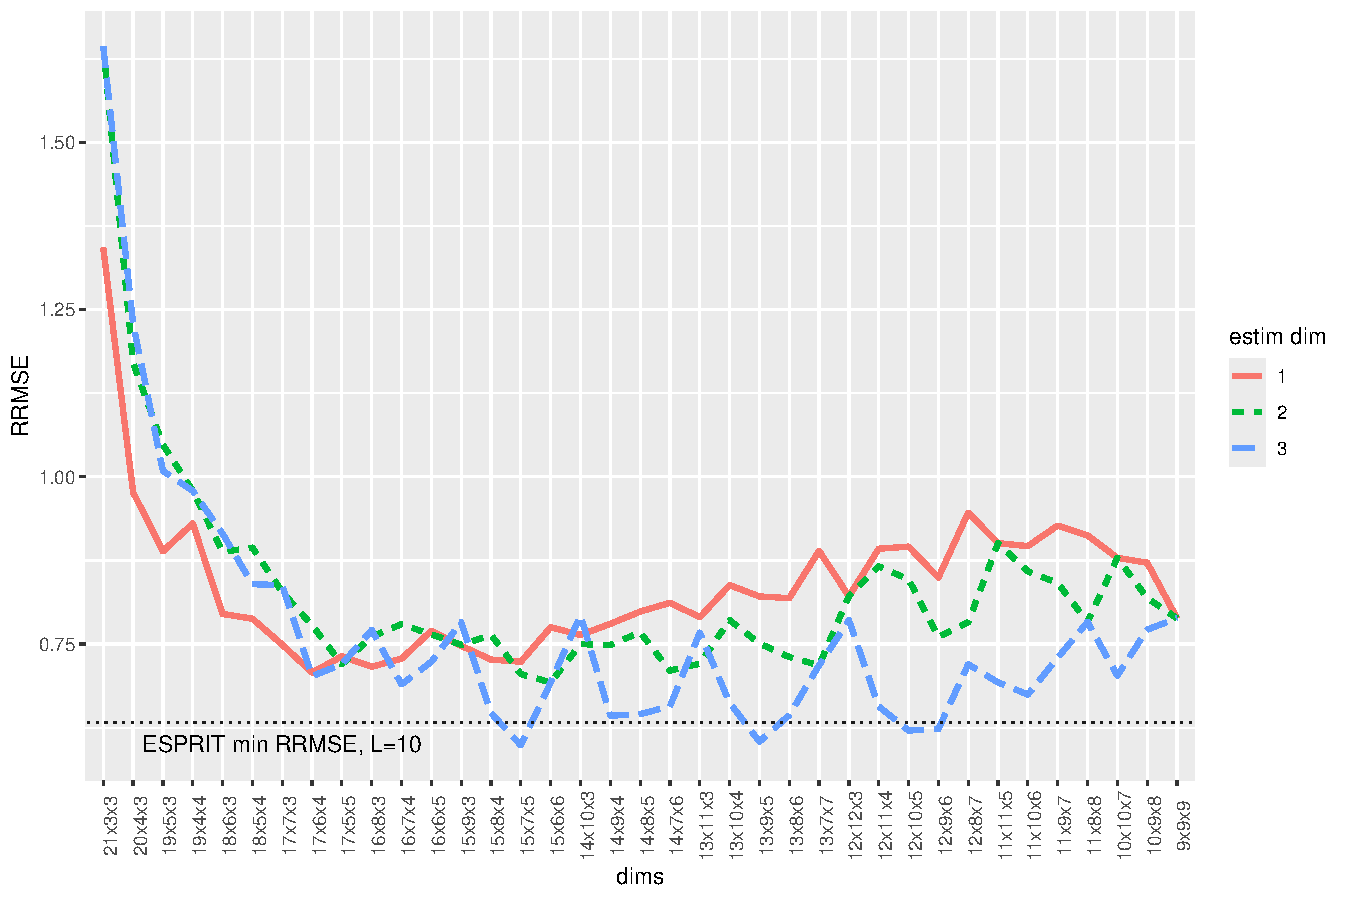
\includegraphics[width=\linewidth]{freq1_dims_no_rates.pdf}
  \caption{Зависимость RRMSE оценки $\omega_1$ от длины окна и направления восстановления.}
  \label{fig:freq1_dims_no_rates}
\end{figure}
\begin{figure}[!ht]
  \centering
  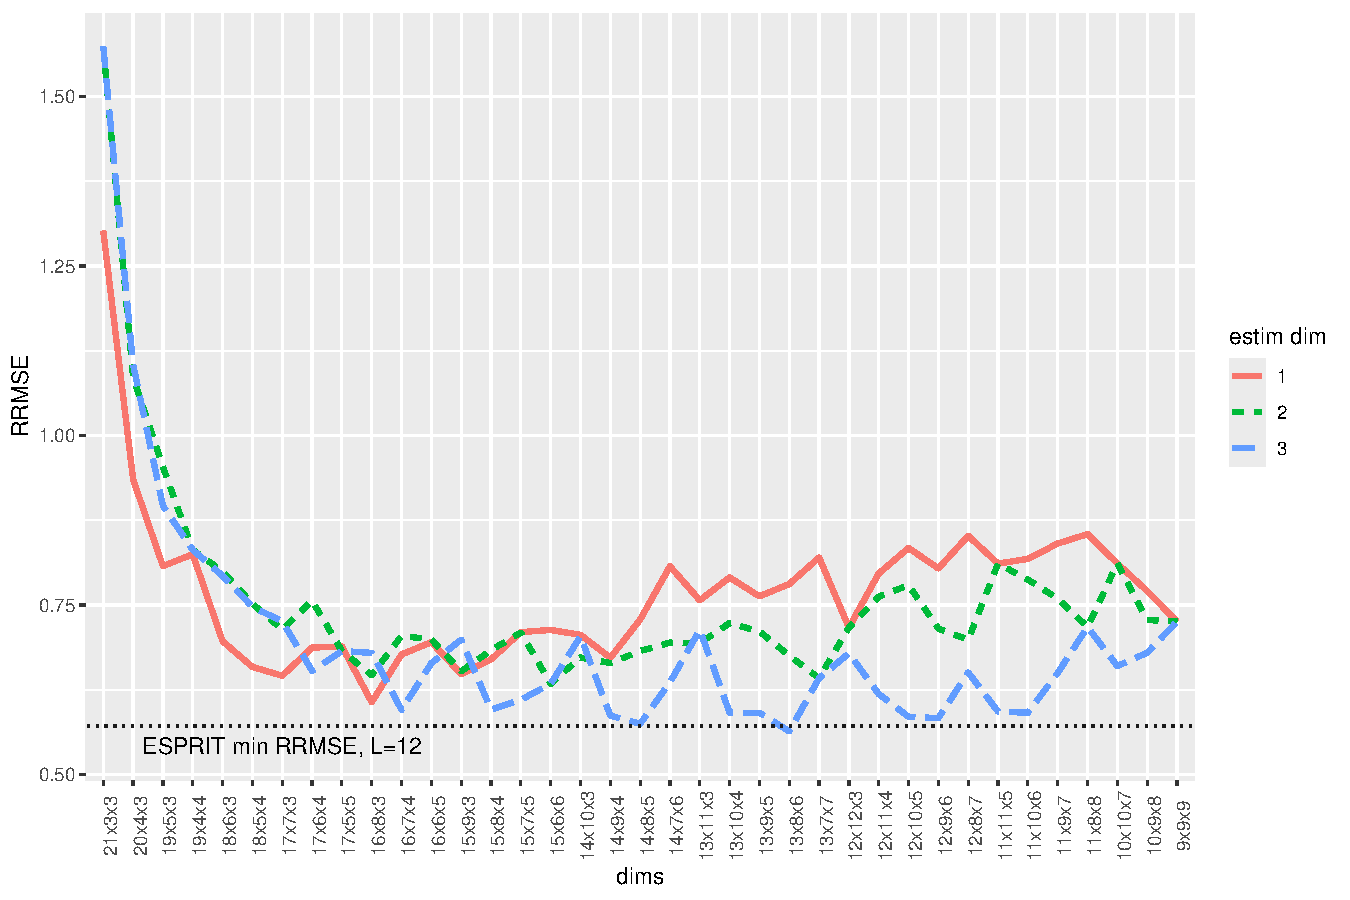
\includegraphics[width=\linewidth]{freq2_dims_no_rates.pdf}
  \caption{Зависимость RRMSE оценки $\omega_2$ от длины окна и направления восстановления.}
  \label{fig:freq2_dims_no_rates}
\end{figure}

\bibliography{main}
\bibliographystyle{ugost2008}
\end{document}
